\documentclass{article}
\usepackage[utf8x]{inputenc}
\usepackage{ucs}
\usepackage{amsmath} 
\usepackage{amsfonts}
\usepackage{marvosym}
\usepackage{wasysym}
\usepackage{upgreek}
\usepackage[english,russian]{babel}
\usepackage{graphicx}
\usepackage{float}
\usepackage{textcomp}
\usepackage{hyperref}
\usepackage{geometry}
  \geometry{left=2cm}
  \geometry{right=1.5cm}
  \geometry{top=1cm}
  \geometry{bottom=2cm}
\usepackage{tikz}
\usepackage{ccaption}
\usepackage{multicol}

\hypersetup{
   colorlinks=true,
   citecolor=blue,
   linkcolor=black,
   urlcolor=blue
}

\usepackage{listings}
%\setlength{\columnsep}{1.5cm}
%\setlength{\columnseprule}{0.2pt}

\usepackage[absolute]{textpos}

\usepackage{colortbl,graphicx,tikz}
\definecolor{X}{rgb}{.5,.5,.5}


\begin{document}
\pagenumbering{gobble}
\lstset{
  language=C,                % choose the language of the code
  basicstyle=\linespread{1.1}\ttfamily,
  columns=fixed,
  fontadjust=true,
  basewidth=0.5em,
  keywordstyle=\color{blue}\bfseries,
  commentstyle=\color{gray},
  stringstyle=\ttfamily\color{orange!50!black},
  showstringspaces=false,
  numbersep=5pt,
  numberstyle=\tiny\color{black},
  numberfirstline=true,
  stepnumber=1,                   % the step between two line-numbers.        
  numbersep=10pt,                  % how far the line-numbers are from the code
  backgroundcolor=\color{white},  % choose the background color. You must add \usepackage{color}
  showstringspaces=false,         % underline spaces within strings
  captionpos=b,                   % sets the caption-position to bottom
  breaklines=true,                % sets automatic line breaking
  breakatwhitespace=true,         % sets if automatic breaks should only happen at whitespace
  xleftmargin=.2in,
  extendedchars=\true,
  keepspaces = true,
}
\lstset{literate=%
   *{0}{{{\color{red!20!violet}0}}}1
    {1}{{{\color{red!20!violet}1}}}1
    {2}{{{\color{red!20!violet}2}}}1
    {3}{{{\color{red!20!violet}3}}}1
    {4}{{{\color{red!20!violet}4}}}1
    {5}{{{\color{red!20!violet}5}}}1
    {6}{{{\color{red!20!violet}6}}}1
    {7}{{{\color{red!20!violet}7}}}1
    {8}{{{\color{red!20!violet}8}}}1
    {9}{{{\color{red!20!violet}9}}}1
}
\section*{Вычислительная сложность. O(n)}
Говорят, что $f(n) = O(n^2)$, если найдутся числа $C$ и $n_0$ такие, что $f(n) < C \cdot n^2$, начиная с  некоторого $n_0$.
\begin{center}
\includegraphics[scale=0.6]{images/On.png}
\end{center}
Другими словами: при больших $n$, $f(n)$ растёт не быстрее чем $n^2$.\\
В информатике за $n$ принимают количество символов во входных данных, а по $y$ лежит время работы или количество элементарных операций алгоритма.

\begin{enumerate}
\item Расположите следующие функции в порядке увеличения скорости роста при больших $n$:
\begin{multicols}{3}
\begin{enumerate}
\item $\log{n}$
\item $1$
\item $\sqrt{n}$
\item $n$
\item $1.001^n$
\item $n!$
\item $n^n$
\item $n\log{n}$
\item $n^2$
\item $2^n$
\end{enumerate}
\end{multicols}

\item Отметьте все функции равные $O(n^2)$
\begin{multicols}{2}
\begin{itemize}
\item $10 n^2$
\item $e^n$
\item $4 n^2 + 10 n + 50$
\item $n!$
\item $n^2 + 10^{-1000} \cdot n^{2.0000000001}$
\item $log(n^9)$
\item $n\log{n}$
\item $n^3 / (1 + n)$
\end{itemize}
\end{multicols}


\item \textbf{} Чему равна средняя вычислительная сложность следующих операций?
\begin{itemize}
\item Нахождение минимального элемента в массиве размера N
\item Нахождение минимального элемента в отсортированном массиве размера N
\item Поиск элемента в массиве размера N
\item Поиск элемента в отсортированном массиве размера N (бинарный поиск)
\item Добавление элемента в начало массива размера N
\item Добавление элемента в конец массива размера N (в предположении, что место под ещё один элемент есть)
\item Сортировка пузырьком массива размера N
\item Сортировка выбором массива размера N
\item Быстрая сортировка массива размера N
\item Добавление элемента в стек с динамическим выделением памяти размера N
\item Удаление элемента из стека размера N
\item Сложение матриц размера  $N \times N$
\item Простой алгоритм умножения матриц размера  $N \times N$
\end{itemize}
\end{enumerate}

\newpage
\section*{Быстрая сортировка - Quicksort}
\begin{multicols}{2}
\begin{lstlisting}
#include <stdio.h>
#include <stdlib.h>
#define N 30

void quicksort(int array[], int lo, int hi)
{
    if (hi - lo > 1)
    {
        int j = lo;
        int pivot = array[hi - 1];
        for (int i = lo; i < hi; i++)
            if (array[i] <= pivot)
            {
                int temp = array[i];
                array[i] = array[j];
                array[j] = temp;
                j++;
            }

        quicksort(array, lo, j - 1);
        quicksort(array, j, hi);
    }
}

void print(int array[], int n)
{
    for (int i = 0; i < n; i++)
        printf("%d ", array[i]);
    printf("\n");
}

int main()
{
    int numbers[N];
    for(int i = 0; i < N; i++)
        numbers[i] = rand() % 100;
    
    print(numbers, N);
    quicksort(numbers, 0, N);
    print(numbers, N);
}
\end{lstlisting}
\vfill\null
\columnbreak
\includegraphics[scale=0.53]{../images/qs2.png}
\\
\\
\\
\includegraphics[scale=0.53]{../images/qs4.png}
\\
\\
\\
\includegraphics[scale=0.53]{../images/qs5.png}
\\
\\
\\
\includegraphics[scale=0.53]{../images/qs6.png}
\\
\\
\\
\includegraphics[scale=0.53]{../images/qs7.png}
\\
\\
\\
\includegraphics[scale=0.53]{../images/qs8.png}
\\
\\
\\
\includegraphics[scale=0.53]{../images/qs9.png}
\\
\\
\\
\includegraphics[scale=0.53]{../images/qs10.png}
\\
\\
\\
\includegraphics[scale=0.47]{../images/qs11.png}
\end{multicols}
\begin{itemize}
\item \textbf{Сравнение сортировок:} Проведите сравнения скорости работы сортировки выбором $O(n^2)$ и быстрой сортировки $O(n \cdot log(n))$. Для этого засеките время работы обеих сортировок при следующих размерах \\
\texttt{N = 100, 1000, 10\textsuperscript{4}, 10\textsuperscript{5}, 10\textsuperscript{6}, 10\textsuperscript{7}}.
Для замера времени используйте утилиту \texttt{time} в терминале:
\begin{verbatim}
time ./a.out
\end{verbatim}
При этом нужно закомметировать печать на экран, так как печать может занимать много времени.\\
Если у Вас не работает утилита \texttt{time}, то есть алтернатива - функция \texttt{clock} из библиотеки \texttt{time.h}:   \\
\href{http://www.cplusplus.com/reference/ctime/clock/}{cplusplus.com/reference/ctime/clock}
\item \textbf{По убыванию:} Измените сортировку \texttt{quicksort}, так, чтобы эта функция сортировала по убыванию.
\item \textbf{По последней цифре:} Измените сортировку \texttt{quicksort}, так, чтобы эта функция сортировала по возрастанию последней цифры.
\item \textbf{Сортировка вещественных чисел:} Измените сортировку \texttt{quicksort}, так, чтобы она сортировала вещественные числа. Проверьте работу сортировки. Для этого сгенерируйте массив из \texttt{N} случайных вещественных чисел от \texttt{0} до \texttt{100} с шагом \texttt{0.01}.
\item \textbf{Города Мира:} В файле \texttt{worldcities.txt} содержится информация о различных городах мира. В каждой строке - информация об одном городе: название города, координаты -  широта(latitude) и долгота(longitude), название страны и население города. В первой строке - общее количество городов.
\begin{itemize}
\item Опишите структуру \texttt{City}, которая будет предназначена для хранения информации об одном городе.
\item \textbf{Считываем города:}\\ Создайте массив из структур \texttt{City} подходящего размера и считайте все данные из файла в массив. Для считывания используйте функцию \texttt{fscanf} из библиотеки \texttt{stdio.h}. Пример считывания:
\begin{lstlisting}
#include <stdio.h>

int main()
{
    // Открываем файл input.txt на чтение("r"). Для открытия на запись - "w"
    FILE* f = fopen("input.txt", "r");
    fscanf(f, < тут всё то же самое, что и у обычного scanf >)
    // ...
    fclose(f);
}
\end{lstlisting}
Учтите, что спецификатор \texttt{\%s} считывает строку до пробела. Чтобы считать строку до запятой используйте спецификатор \texttt{\%[\textasciicircum,]} - при этом \texttt{s} на конец спецификатора ставить не надо.\\
Вся строка для \texttt{fscanf} будет выглядеть следующим образом:
\texttt{``\%[\textasciicircum,],\%f,\%f,\%[\textasciicircum,],\%d\textbackslash n''}

\item \textbf{Сохраняем города:}\\ Написать функцию \texttt{void save\_cities(char filename[], City array[], int n)}, которая будет сохранять города из массива \texttt{array} в файл, чьё название хранится в переменной \texttt{filename}. Например, при вызове \texttt{save\_cities(``output.txt'', cities, n);} массив \texttt{cities} должен сохраниться в файл \texttt{output.txt}.

\item \textbf{По населению:}\\ Создайте функцию \texttt{quicksort\_population}, чтобы она принимала на вход массив из структур \texttt{City} и сортировала их по возрастанию населения. Проверьте функцию в \texttt{main}, отсортировав структуру и сохранив её в файл \texttt{sorted\_by\_population.txt} с помощью функции \texttt{save\_cities}.

\item \textbf{По широте:}\\ Создайте функцию \texttt{quicksort\_latitude}, чтобы она сортировала массив городов по широте - от самого южного города к самому северному. Проверьте функцию в \texttt{main}, отсортировав структуру и сохранив её в файл \texttt{sorted\_by\_latitude.txt}.

\item \textbf{По названию:}\\ Создайте функцию \texttt{quicksort\_name}, чтобы она сортировала массив городов по названию города. Проверьте функцию в \texttt{main}, отсортировав структуру и сохранив её в файл \texttt{sorted\_by\_name.txt}. Используйте функцию \texttt{strcpy} из библиотеки \texttt{string.h}.
\end{itemize}
\end{itemize}

\newpage
\section*{Bogosort}
Bogosort - крайне неэффективная сортировка, состоящая из двух шагов:
\begin{enumerate}
\item Перемешать массив случайным образом.
\item Проверить, отсортирован ли массив, и, если нет, то перейти к шагу 1.
\end{enumerate}
В файле \texttt{1bogosort.c} содержится реализация этой сортировки.
\begin{itemize}
\item Скомпилируйте эту программу (\texttt{gcc -std=c99 1bogosort.c}) и запустите. Попытайтесь отсортировать массив из 10-ти чисел с помощью этой сортировки.
\item Какова вычислительная сложность этой сортировки? Какое среднее число итераций нужно произвести, чтобы отсортировать 10 чисел.
\end{itemize}

\section*{Сортировка подсчётом - Counting Sort}
Быстрая сортировка и некоторые другие хорошие алгоритмы сортировки работают за $O(n \cdot log(n))$. Такая сложность является оптимальной, если ничего больше неизвестно о сортируемых числах. Однако, если о числах что-нибудь известно, то можно добиться лучшего результата. Предположим, что наш массив состоит только из нулей и единиц и имеет примерно такой вид: \\
\texttt{int array[] = \{0, 0, 1, 0, 0, 0, 1, 1, 0, 1, 1, 1, 1, 1, 1, 0, 1, 0, 0, 0, 0, 0, 0, 0, 1, 1, 0, 1, 1, 0, 0, 0, 0, 0, 1, 0, 1, 0, 1, 1, 0, 0, 1, 0, 0, 0, 1, 0, 0, 0, 0, 1, 1, 1, 0, 0, 0, 1, 0, 0, 1, 1, 1, 1, 0, 0, 1, 1, 0, 0, 0, 1, 1, 1, 0, 1, 1, 1, 1, 0, 1, 0, 1, 0, 0, 1, 1, 0, 0, 1, 0, 1, 1, 0, 1, 0, 0, 1, 1, 1, 1, 0, 0, 0, 1, 1, 0, 1, 0, 0, 0, 0, 1, 1, 0, 1, 0, 1, 1, 0, 0, 0, 0, 0, 0, 1, 1, 0, 1, 1, 0, 1, 1, 0, 1, 0, 0, 1, 0, 0, 1, 1, 0, 1, 1, 1, 1, 0, 1, 0, 1, 1, 1, 0, 1, 1, 1, 1, 0, 0, 0, 0, 0, 0, 1, 0, 1, 0, 0, 0, 1, 1, 1, 0, 0, 1, 1, 0, 0, 0, 1, 0, 1, 1, 0, 0, 0, 0, 1\}}\\
Как отсортировать массив, состоящий только из нулей и единиц, за $O(n)$?\\
Напишите сортировку подсчётом для сортировки однозначных чисел (файл \texttt{2countsort.c}).\\
Можно ли сортировать таким методом массивы, содержащие большие числа?\\
Какова будет вычислительная сложность данного алгоритма для сортировки $n$ положительных чисел, которые могут принимать значения от $0$ до $k$.

\section*{Цифровая сортировка - Radix Sort}
Цифровая сортировка заключается в последовательном применении сортировок подсчётом к цифрам числа. То есть, сначала сортируем весь массив по последней цифре, потом по предпоследней и т. д. При этом, важно, чтобы сортировка подсчётом сохраняла порядок элементов с одинаковыми цифрами.
\begin{itemize}
\item Какова вычислительная сложность данного алгоритма.
\item Реализуйте алгоритм цифровой сортировки и сравните его с быстрой сортировкой.
\end{itemize}
\newpage


\if false
\subsection*{Стандартная функция qsort()}

Пример использования функции qsort():
\begin{verbatim}
#include <stdio.h>      /* printf */
#include <stdlib.h>     /* qsort */

int cmp(const void* a, const void* b)
{
    int* pa = (int*)a;
    int* pb = (int*)b;
    return ( *pa - *pb );
}

int main ()
{
    int arr[] = {163, 624, 7345, 545, 41, 78, 5, 536, 962, 1579};
    qsort(arr, 10, sizeof(int), cmp);
   
    print_array(10, arr);
}
\end{verbatim}


\subsubsection*{Задачи:}
\begin{enumerate}
\item Отсортировать числа массива \texttt{arr} по убыванию.
\item Отсортировать числа массива \texttt{arr} по возрастанию последней цифры.
\item Отсортировать числа массива \texttt{arr} по первой цифре числа.
\item Описать структуру \texttt{Movie} с полями \texttt{title}(название -- строка), \texttt{year}(год выхода -- целое число), \texttt{rating}(рейтинг на кинопоиске -- вещественное число). Создать массив из 6-ти таких структур. Написать отдельную функцию для печати такого массива на экран.
\item Отсортировать массив фильмов по убыванию рейтинга. 
\item Отсортировать массив фильмов по возрастанию года выхода. 
\item Интерпретируем значения массива \texttt{arr}, как значения некоторых углов в градусах. Отсортировать числа по возрастанию косинусов соответствующих углов.
\item Отсортировать числа массива \texttt{arr} следующим образом: сначала четные числа по возрастанию, затем нечётные по убыванию.
\end{enumerate}

\fi


\end{document}